\section{Proposed Method}
% -----------------------------------------------------------------------

\subsection{Core Idea}

The central question of this work is: \emph{when should a listener ask a
clarifying question rather than commit to an answer?} 

Concretely, given a posterior $P(t\mid u)$ over $N$ candidate objects, the
listener's two actions have expected utilities:
\begin{align}
  \text{EU}(\text{commit}) &= \max_i\, P(t_i \mid u), \label{eq:eu-commit}\\
  \text{EU}(\text{ask})    &= 1 - c, \label{eq:eu-ask}
\end{align}
where $c\in(0,1)$ is the per-question cost.  The listener commits when
$\text{EU}(\text{commit}) \geq \text{EU}(\text{ask})$, i.e.\
\begin{equation}
  \max_i P(t_i\mid u) \;\geq\; 1 - c.
  \label{eq:eu-rule}
\end{equation}

Figure~\ref{fig:pipeline} illustrates the full two-agent pipeline.  The
\textbf{speaker} is given the target object's attributes and produces a
referring utterance $u$.  The \textbf{listener} observes the scene and $u$,
computes a posterior, and applies the EU rule.  If the rule triggers asking,
the listener emits a yes/no clarification question; an oracle answers; the
listener updates its posterior and may ask again (up to two turns); it then
commits.

\begin{figure}[H]
\centering
\begin{tikzpicture}[
  node distance = 4mm and 10mm,
  box/.style  = {draw, rounded corners=4pt, fill=#1,
                 text width=2.5cm, align=center,
                 minimum height=1.2cm, font=\small, inner sep=6pt},
  box/.default = white,
  sbox/.style = {draw, rounded corners=4pt, fill=#1, dashed,
                 text width=2.5cm, align=center,
                 minimum height=1.2cm, font=\small, inner sep=6pt},
  sbox/.default = white,
  arr/.style  = {-{Stealth[length=2.4mm]}, thick},
  labl/.style = {font=\scriptsize\itshape, midway,
                 fill=none, fill opacity=0.85, text opacity=1,
                 rounded corners=2pt, inner sep=2pt},
]

%% ── TOP ROW ─────────────────────────────────────────────────────────────
\node[] (scene-base) {};
\node[box=blue!15, xshift=-15mm]   (scene)  {Scene $\mathcal{S}$\\\footnotesize $N$ objects};
\node[box=orange!25, right=of scene-base] (spk)    {Speaker\\\footnotesize (knows target)};
\node[box=green!20,  right=of spk]   (lst)    {Listener\\\footnotesize posterior $P(t_i{\mid}u)$};
\node[box=yellow!30, right=of lst]   (eu)     {EU Rule\\\footnotesize $\max P \geq 1{-}c$?};

%% ── BOTTOM ROW ──────────────────────────────────────────────────────────
\node[box=green!35,  below=20mm of eu]   (commit) {Commit\\\footnotesize $\hat{t}=\arg\max_i P$};
\node[sbox=red!15,   below=20mm of lst]  (ask)    {Ask\\\footnotesize yes/no question};

%% ── MAIN FLOW ───────────────────────────────────────────────────────────
\draw[arr] (scene) -- node[labl,above]{target attrs}  (spk);
\draw[arr] (spk)   -- node[labl,above]{$u$}            (lst);
\draw[arr] (lst)   -- node[labl,above]{posterior}      (eu);

%% scene image also feeds listener (arc below)
\draw[arr] (scene.south) -- ++(0,-8mm) -|
    node[labl,below,pos=0.1]{scene image with indices} (lst.south);

%% ── EU BRANCHES ─────────────────────────────────────────────────────────
\draw[arr] (eu.south)  -- node[labl,right]{\textbf{yes}} (commit.north);
\draw[arr] 
    (eu.south)
    -- ++(-8mm,0)
    |- ++(0,-10mm)
    -| node[labl,right,pos=0.6]{\textbf{no}}
    (ask.north);

%% ── DIALOGUE LOOP: listener asks speaker, speaker answers ───────────────
\draw[arr] (ask.west) -- ++(0,0mm) -|
    node[labl,above,pos=0.25]{question} (spk.south);

%% ── BACKGROUND PANELS ───────────────────────────────────────────────────
\begin{scope}[on background layer]
  \node[fill=orange!8, draw=orange!50, rounded corners=7pt,
        fit=(scene)(spk), inner sep=8pt,
        label={[font=\footnotesize\bfseries,orange!80!black]above:Speaker}] {};
  \node[fill=blue!5, draw=blue!35, rounded corners=7pt,
        fit=(lst)(eu)(commit)(ask), inner sep=8pt,
        label={[font=\footnotesize\bfseries,blue!70!black]above:Listener}] {};
\end{scope}

\end{tikzpicture}
\caption{The cost-aware reference game pipeline.  The speaker knows the target
and generates a referring utterance $u$.  The listener computes a posterior
and applies the EU rule (Eq.~\ref{eq:eu-rule}).}
\label{fig:pipeline}
\end{figure}

\subsection{Task and Data}

A \textbf{scene} $\mathcal{S} = \{o_1,\ldots,o_N\}$ contains $N$ objects,
each described by four discrete attributes:
\begin{enumerate}
  \item \texttt{color} $\in\{\text{red, blue, green, yellow, purple, orange}\}$,
  \item \texttt{shape} $\in\{\text{circle, square, triangle}\}$,
  \item \texttt{size} $\in\{\text{small, medium, large}\}$, and
  \item a continuous 2-D position $(x,y)\in[0,100]^2$
        (bottom-left origin; $y$ increases upward).
\end{enumerate}
One object is designated the \textbf{target} $t \in \mathcal{S}$; all others
are \textbf{distractors}.  We generate scenes with $N\in\{6,8,10\}$ under two
overlap conditions.  In the \texttt{none} condition, there would be no spatial overlapping between the objects.
In the \texttt{force} condition, objects are forced to be overlapping. Scene images are rendered at $512\times512$ pixels using PIL.  (see Appendix~\ref{fig:scene-example})
Each $(N,\text{condition})$ pair contains 100 fixed scenes; all speaker and listener strategies see the same 100 scenes, giving 600 unique scenes in total. 

\subsection{Speaker Strategies}
\label{sec:speakers}

The speaker receives the target's attributes as plain text (not a visual
annotation) to avoid color hallucination on the rendered image. 
We implement eight distinct strategies:

\begin{table}[H]
\centering
\small
\begin{tabular}{lp{10.8cm}}
\toprule
\textbf{Speaker} & \textbf{Description} \\
\midrule
\texttt{feature\_canonical} & Rule-based; enumerates color and shape, then adds size and/or location only if needed for uniqueness. No LLM call. \\[4pt]
\texttt{natural} & LLM generates a free-form referring expression
  (e.g., ``the green circle at the bottom left''). \\[4pt]
\texttt{pragmatic} & LLM is prompted to be maximally informative while remaining concise; produces RSA-style level-1 pragmatic descriptions. \\[4pt]
\texttt{scene\_first} & LLM receives the full distractor list and produces the shortest uniquely identifying description. \\[4pt]
\texttt{listener\_aware} & LLM is told the listener can see an annotated scene image; crafts descriptions that exploit spatial landmarks. \\[4pt]
\texttt{landmark} & LLM identifies a salient landmark object and describes the target as a spatial relation to it (e.g., ``to the left of the large red square''). \\[4pt]
\texttt{contrastive} & LLM identifies the most confusable distractor (foil) and produces a contrastive description highlighting the distinguishing feature. \\[4pt]
\texttt{superlative} & LLM uses uniqueness or superlative descriptions (``the only triangle'', ``the largest red object''). \\
\bottomrule
\end{tabular}
\caption{Speaker strategies.}
\label{tab:speakers}
\end{table}

All LLM-based speakers use \texttt{gemini-2.0-flash-001} via the OpenRouter
API.  Speaker utterances are cached per (scene, speaker) to avoid redundant
API calls; once generated, the same utterance is reused across all listener
evaluations.

\subsection{Listener Strategies and Posterior Computation}
\label{sec:listeners}

The listener receives the utterance $u$ together with an index-annotated scene
image.  Its goal is to produce a probability distribution $P(t_i\mid u)$ over all $N$
objects.

We implement six listener backends that differ in \emph{how} they compute
the posterior (Table~\ref{tab:listeners}).  Five listeners
(\texttt{index}, \texttt{direct}, \texttt{cot}, \texttt{elimination},
\texttt{feature-match}) directly emit a probability vector over object indices.
The \texttt{coordinate} listener instead predicts a 2-D point $(\hat{x},
\hat{y})$ in scene coordinates, then converts the prediction to a posterior via
a Gaussian distance kernel:
\begin{equation}
  P(t_i\mid u) \;\propto\;
  \exp\!\left(-\frac{\|\,(\hat{x},\hat{y}) - (x_i,y_i)\,\|^2}{2\sigma^2}\right),
  \quad \sigma = 10.
  \label{eq:gauss-kernel}
\end{equation}
The bandwidth $\sigma{=}10$ (on the $[0,100]^2$ grid) was chosen so that a
prediction landing squarely on an object assigns $\geq 0.97$ probability to
that object when $N{=}6$; predictions that fall between two nearby objects
produce a bimodal posterior that correctly reflects ambiguity.  No temperature
parameter is tuned; the kernel is fixed across all conditions.

\begin{table}[H]
\centering
\small
\begin{tabular}{lp{10.8cm}}
\toprule
\textbf{Listener} & \textbf{Description} \\
\midrule
\texttt{index} & Single-pass: outputs a single index as the final answer. \\[4pt]
\texttt{direct} & Outputs probabilities over indices. \\[4pt]
\texttt{cot} & Chain-of-thought: first describes each indexed object, then scores each, then normalises. \\[4pt]
\texttt{elimination} & Sequentially eliminates objects inconsistent with the utterance; posterior is uniform over survivors. \\[4pt]
\texttt{feature\_match} & Parses utterance into attribute tokens; soft-matches each token against object attributes to form a score vector. \\[4pt]
\texttt{coordinate} & Predicts a 2-D coordinate $(\hat x, \hat y)$ and converts to a posterior via Eq.~\ref{eq:gauss-kernel}. \\
\bottomrule
\end{tabular}
\caption{Listener strategies evaluated in this work.}
\label{tab:listeners}
\end{table}

When the EU rule triggers asking, the listener generates a yes/no clarification
question which is posed directly to the speaker.  The speaker answers
deterministically from the ground-truth target attributes.  The posterior is
then updated by zeroing out objects inconsistent with the answer and
renormalizing, and the EU rule is re-evaluated; this repeats for up to two
turns before the listener commits.

\subsection{Evaluation Metrics}
\label{sec:metrics}

\textbf{Accuracy} is the fraction of \emph{all} $n$ scenes in which the
listener identifies the correct target.
\textbf{Clarification Rate} (ask\%) is the fraction of scenes where at least
one question is asked.  \textbf{Cost-Penalised Accuracy} (CPA) rewards
correct answers and penalises questions:
\begin{equation}
  \text{CPA} = \text{Accuracy} - c \times \text{ask\%}.
  \label{eq:cpa}
\end{equation}

% We also report the mean \textbf{Brier Score}
% $\text{BS} = \frac{1}{N}\sum_{i=1}^{N}(p_i - y_i)^2$,
% where $y_i{=}1$ iff object $i$ is the target, as a calibration proxy for
% the posterior quality.  Lower is better; a perfectly peaked posterior on the
% correct object gives $\text{BS} = 0$.

% -----------------------------------------------------------------------
\section{Experiment Results}
% -----------------------------------------------------------------------
\label{sec:results}

We evaluate 28{,}800 trials over speaker$\times$listener$\times$scene-size$\times$condition
configurations at $c{=}0.25$. 

% -----------------------------------------------------------------------
\subsection{Free-form speakers are more robust to scale than
            structured speakers, while landmark descriptions collapse}

Figure~\ref{fig:speaker_scaling} shows listener accuracy for all eight
speakers with the \texttt{index} listener across $N\in\{6,8,10\}$ objects
under both overlap conditions.

\begin{figure}[H]
  \centering
  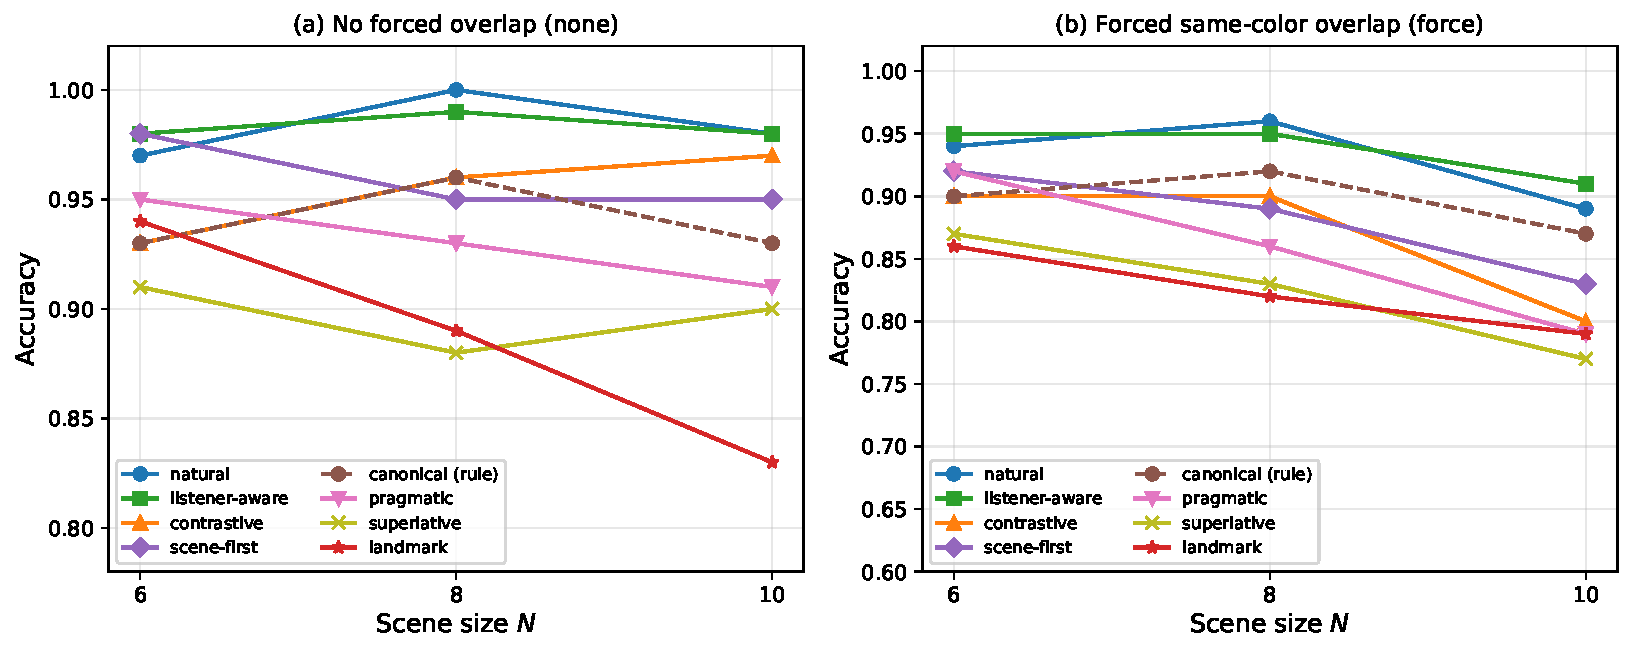
\includegraphics[width=0.9\linewidth]{../figures/fig1_speaker_scaling.pdf}
  \caption{Accuracy vs.\ scene size for all eight speaker strategies,
           using the \texttt{index} listener at $c{=}0.25$.
           Left: no forced overlap (\texttt{none}); right: forced
           same-color distractor (\texttt{force}).
           Marker size is uniform; line styles distinguish speakers.}
  \label{fig:speaker_scaling}
\end{figure}

\begin{table}[H]
\centering
\small
\label{tab:main-results}
\setlength{\tabcolsep}{7pt}
\begin{tabular}{lccc}
\toprule
Speaker & $N{=}6$ & $N{=}8$ & $N{=}10$ \\
\midrule
\texttt{natural}         & 0.970 & \textbf{1.000} & \textbf{0.980} \\
\texttt{listener\_aware} & \textbf{0.980} & 0.990 & \textbf{0.980} \\
\texttt{contrastive}     & 0.930 & 0.960 & 0.970 \\
\texttt{scene\_first}    & \textbf{0.980} & 0.950 & 0.950 \\
\texttt{feature\_canonical}         & 0.930 & 0.960 & 0.930 \\
\texttt{pragmatic}       & 0.950 & 0.930 & 0.910 \\
\texttt{superlative}     & 0.910 & 0.880 & 0.900 \\
\texttt{landmark}        & 0.940 & 0.890 & 0.830 \\
\midrule
Uniform baseline & 0.167 & 0.125 & 0.100 \\\bottomrule
\end{tabular}
\caption{Speaker comparison with the \texttt{index} listener, $c{=}0.25$, \texttt{none} condition.  Since ask\% $= 0$ for all, CPA $=$ Accuracy. Best per column in \textbf{bold}.}
\end{table}

\textbf{\texttt{natural} and \texttt{listener\_aware} are
the most robust speakers.}  Both maintain $\geq0.97$ accuracy at $N{=}10$
(none), with \texttt{natural} achieving a perfect $1.000$ at $N{=}8$.
These speakers generate concise, spatially grounded descriptions that
uniquely identify the target even in dense scenes.  The rule-based
\texttt{feature\_canonical} is competitive ($0.93$--$0.96$) with zero LLM
calls, matching or exceeding LLM-based pragmatic and landmark speakers.

\textbf{Landmark descriptions collapse at large $N$.}
\texttt{landmark} drops from $0.940$ at $N{=}6$ to $0.830$ at
$N{=}10$ on the \texttt{none} condition ($\Delta{=}-0.110$), and further
to $0.650$ on the \texttt{force} condition at $N{=}10$.  This failure is
systematic: with more objects, a landmark that is itself described by
color+shape becomes ambiguous (two yellow circles), creating a cascading
reference failure.  \texttt{superlative} shows a smaller but
consistent degradation from $0.910\to0.900$.

\textbf{Forced overlap is a clean difficulty dial.}  Under \texttt{force},
all speakers degrade (average $\Delta{=}-0.045$ at $N{=}8$), but the
rank ordering is preserved: the best-performing speakers on \texttt{none}
remain best on \texttt{force}. 

% -----------------------------------------------------------------------
\subsection{Listener strategy determines the
            accuracy--cost trade-off; ask rate is the dominant CPA penalty}

Figure~\ref{fig:listener_scatter} plots accuracy against ask rate for all
listener strategies paired with the \texttt{feature\_canonical} speaker.
Each point is one (listener, $N$) configuration; iso-CPA lines are overlaid.
\emph{Ideal listeners occupy the top-left corner} (high accuracy, low ask).

\begin{figure}[H]
  \centering
  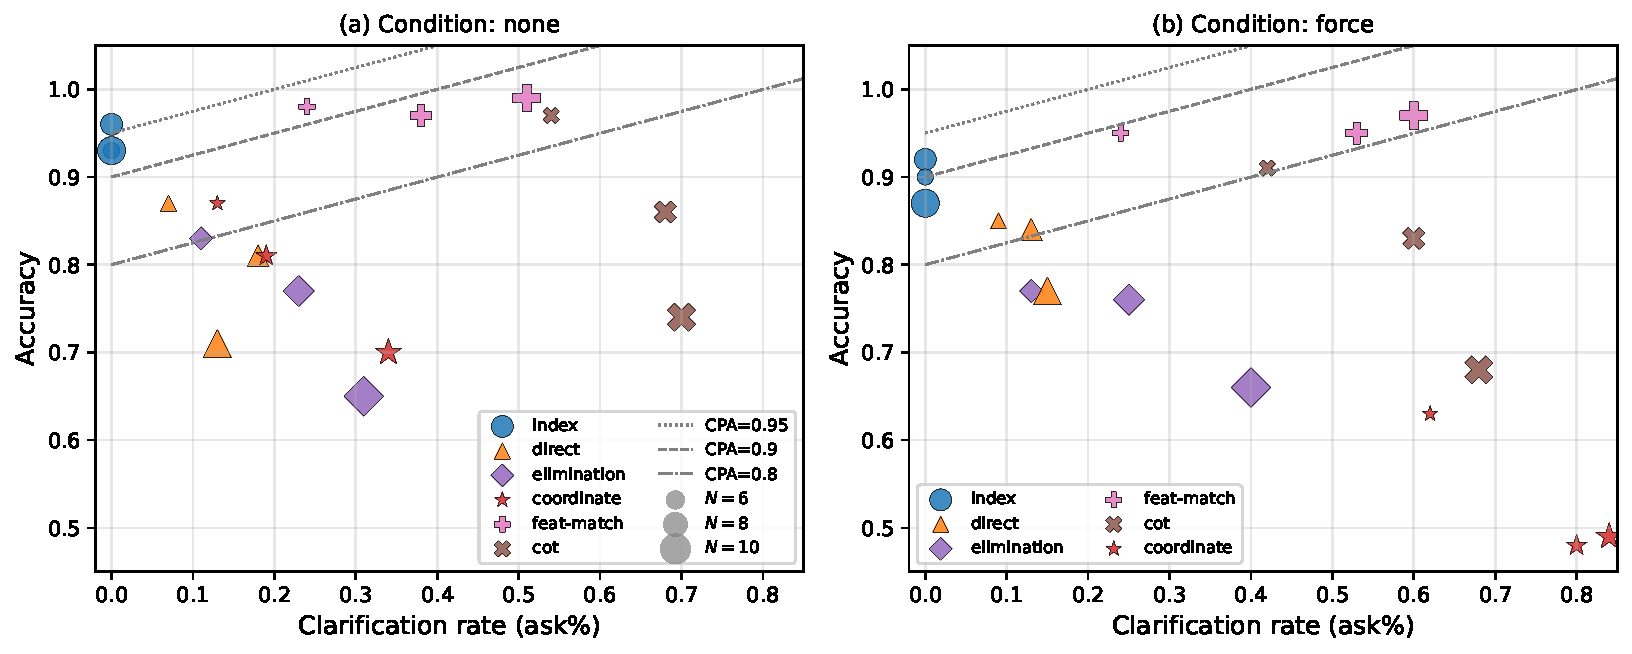
\includegraphics[width=\linewidth]{../figures/fig2_listener_scatter.pdf}
  \caption{Accuracy vs.\ clarification rate for all listener strategies,
           \texttt{feature-canonical} speaker, $c{=}0.25$.
           Point size encodes scene size $N\in\{6,8,10\}$.
           Dashed/dotted lines are iso-CPA contours.}
  \label{fig:listener_scatter}
\end{figure}

\begin{table}[t]
\centering
\small
\label{tab:listener-comparison}
\setlength{\tabcolsep}{5pt}
\begin{tabular}{lcccccc}
\toprule
\multirow{2}{*}{Listener} &
\multicolumn{3}{c}{\texttt{none}} &
\multicolumn{3}{c}{\texttt{force}} \\
\cmidrule(lr){2-4}\cmidrule(lr){5-7}
 & Acc & Ask\% & CPA & Acc & Ask\% & CPA \\
\midrule
\texttt{index}         & \textbf{0.960} & 0.00 & \textbf{0.960} & \textbf{0.920} & 0.00 & \textbf{0.920} \\
\texttt{direct}        & 0.810 & 0.18 & 0.765 & 0.840 & 0.13 & 0.807 \\
\texttt{elimination}   & 0.770 & 0.23 & 0.713 & 0.760 & 0.25 & 0.698 \\
\texttt{feature-match} & 0.970 & 0.38 & 0.875 & 0.950 & 0.53 & 0.817 \\
\texttt{coordinate} & 0.810 & 0.19 & 0.763 & 0.480 & 0.80 & 0.280 \\
\texttt{cot}           & 0.860 & 0.68 & 0.690 & 0.830 & 0.60 & 0.680 \\
\bottomrule
\end{tabular}
\caption{Listener comparison with \texttt{feature-canonical} speaker, $c{=}0.25$, $N{=}8$.}
\end{table}

\textbf{The \texttt{index} listener dominates in CPA by never asking.}
Its structured attribute-table input eliminates all referential ambiguity
in the text channel: the posterior saturates to $\max_i P \approx 1.0$
at every scene, so the EU rule never fires.  CPA equals accuracy ($0.960$
at $N{=}8$, none), the highest of any listener.

\textbf{CoT reasoning inflates ask rate to $>60\%$, substantially reducing CPA.}
Despite achieving accuracy comparable to the top listeners (0.860 at $N{=}8$),
the \texttt{cot} listener's CPA is only 0.690 because it asks on 68\% of scenes.
Each time the model verbalises visual uncertainty (``Object 3 appears either
blue or green''), the resulting posterior approaches uniform, triggering the
EU rule even when the underlying argmax would have been correct.  This is the
largest CPA gap of any listener strategy---a $-0.270$ drop from \texttt{index}
to \texttt{cot}---and illustrates that expressed calibration harms the
clarification rule.

\textbf{\texttt{coordinate} degrades catastrophically under forced overlap.}
On \texttt{none}, \texttt{coordinate} achieves 0.810 accuracy and 0.763 CPA,
comparable to \texttt{direct}.  On \texttt{force}, accuracy falls to 0.480
and CPA drops to $0.280$ as the ask rate rises to 80\%.
When a same-color distractor sits nearby, the predicted coordinate falls
between target and foil, producing a flat Gaussian posterior that perpetually
triggers clarification---but yes/no answers cannot resolve a coordinate
prediction error.  The \texttt{feature-match} listener shows a similar
pattern: very high accuracy ($0.950$--$0.970$) but excessive asking
($38\%$--$53\%$), yielding CPA of $0.875$/$0.817$ (none/force) well below
its accuracy, confirming that posterior flatness need not correspond to
genuine referential ambiguity.

